\section{Introduction}
This paper is about an academic project born to be an efficient solution for the CINI\footnote{Consorzio Interuniversitario Nazionale per l'Informatica} 2017 Challenge on smart cities illumination system. In particular, the goal was to prototype and test a solution which was capable of (near) real-time data stream processing for monitoring records from street lamps, lumen sensors co-located with the street lamps themselves and from traffic data produced by third-party APIs. We will explore this solution for the following use case: in a smart city context it is necessary to guarantee the maximum efficiency from lamps consumption while providing an optimal illumination within safety limits for pedestrians and drivers according to local traffic intensity. To achieve that, it is necessary to project a grid of smart lamps capable of tuning their light level according to the right amount of energy necessary to provide city aware, safe and green consumption levels. This grid must be powered and managed via a reliable, highly available, processing-capable control system. Introducing Project Ember.

\section{Frameworks and Tools}
We structured our environment using at first a publish/subscribe architecture with street lamps, lumen and traffic sensors as publishers and a stream processing framework as subscriber. 

\subsection{Data stream processing}
The Apache Software Foundation makes available different alternatives, each one a refined version of the previous. We chose Apache Flink\footnote{Apache Flink official page: https://flink.apache.org/} which is the most recent data stream processing platform. Flink gives the programmer the possibility to define just the topology of the operators, how they are linked, or how to set the windows timing (based upon the event time or upon the processing time spent inside the system). Flink handles the under-the-hood engine: multithreading, synchronization, parallelism, availability, cluster management. We chose the latest stable release of Apache Flink, 1.2.0, which comes with a well written documentation as well as multiple connectors for the most popular MOM\footnote{Messages Oriented Middleware} and storages. Flink calls a \texttt{Source} the very component that produces data and \texttt{Sink} the one that takes the processed data in order to store or to route them to another entity.

\subsection{Connectors}
To achieve scalability we had to analyze several options to connect our Flink topology to messages routers and to the persistence level. The MOM chosen was Apache Kafka\footnote{Apache Kafka documentation: https://kafka.apache.org/documentation} which works seamlessly with Flink thanks to the included connector plugins, giving the possibility to simply customize the connection according to our preferences: in this solution Kafka is our preferred \texttt{Source} to handle data from the sensors. 
\subsection{Persistence level}
A NoSQL approach was mandatory to us, to collect dynamic unstructured data typical of a sensor network, so we analyzed different products: in particular Elasticsearch\footnote{Elasticsearch official page: https://www.elastic.co/products/elasticsearch} and Apache Cassandra. We chose Elasticsearch, as it is fully supported (although not its last version) by Flink 1.2.0 and it is a flexible, easy-to-deploy database with RESTful APIs. It leverages the ability to perform complex queries, even geographical and lexical ones, with good performances and scalability options. Elasticsearch is part of the Elastic Stack which makes available another useful tool for visualizing stored data, Kibana\footnote{Kibana official page: https://www.elastic.co/products/kibana}.

\subsection{Extras}
To develop a local control unit to manage the city grid we used Flask and Redis. Flask\footnote{Flask official page: http://flask.pocoo.org/} is a micro-framework for web server built in Python and Redis\footnote{Redis official page: https://redis.io/} is a simple and efficient key-value data store which can work as a database, cache or message broker. Redis serves us as a cache, allowing us to interact with control unit history with very simple APIs via the endpoints exposed by Flask.

\subsection{Programming languages}
Java\footnote{1.8 update 121} is the programming language that links all these components together being used by Flink (which supports Scala as well) and Elasticsearch connector. We also used Python for the control unit development as well as to realize the simulated data source for testing.


\section{Architecture overview}
In this section we will cover how the system communicates between each of its components and modules and the assumptions we made to prototype the architecture. In \hyperref[fig:ember_architecture]{figure 1} a high-level overview is provided. Before proceeding, we want to focus on the output from the real-time\footnote{We will define the system as "real-time" in this paper even if is not validated for such a control system, but it is capable of near real-time data stream processing} control system: it is produced into the MOM and consumed by control units, closing a feedback loop. This behavior and the capability to maintain high-availability across the clusters make the system itself near to the features of an autonomic system.
\begin{figure}[!b]
\begin{center}
	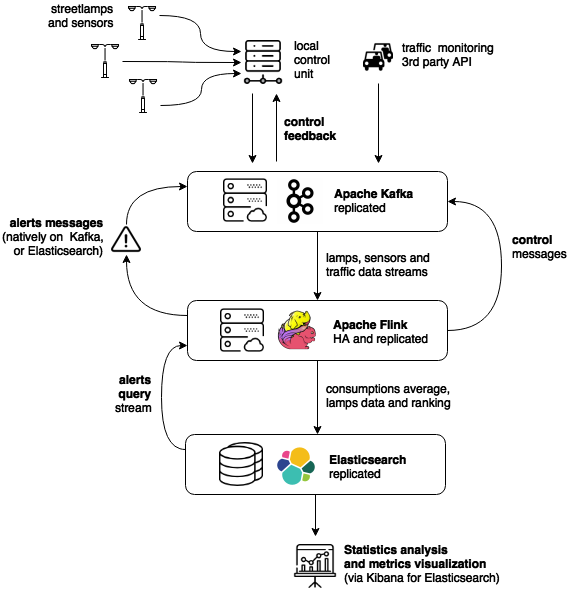
\includegraphics[scale=0.35]{img/ember_architecture}
	\caption{Project Ember architecture overview}
	\label{fig:ember_architecture}
\end{center}
\end{figure}

\subsection{A Message Oriented Approach}
First of all let us consider how the sensors network sends its data to the control system. According to project specifications the street lamps send to the system JSON formatted strings, containing all the information their micro-controllers collect, as tuples. Lamps are able to connect to the city intranet, to understand the power level proper of the bulb model and how such parameters relates one another in order to obtain the right luminosity.
 A lumen sensor is placed upon the street lamp and it sends data every 10 seconds giving us information about the daylight luminosity level and the lamp's ID, all handled by the same micro-controller.
 A traffic intensity API is available to produce a continuous stream of records maintaining an address indicator and a traffic percentage. All of these data are sent every 10 seconds.

\subsection{Apache Kafka cluster}
 Apache Kafka plays its MOM role connecting all the components of our system so they can relate each other. Such a system is sufficient to build a prototype but let’s analyze better the problem: the system, a smart lamps grid, has to emit orders directed to a single lamp among thousands. Kafka can manage runtime topics creation but a topic for each lamp is meaningless and inefficient; requiring the data stream processing system to know the right position of the lamp among network is infeasible as well: we will use control units identifiers.
To handle the thousands of data necessary to manage the infrastructure, we thought to use a cluster of replicated nodes running the same Apache Kafka instance, using Apache Zookeeper\footnote{Apache Zookeeper official page: https://zookeper.apache.org} to maintain the cluster available via redirection from a public IP. The MOM allows us to register topics for lamps, sensors and traffic monitoring data to retrieve them as a stream in Flink, and automatically creates topics for each control unit in order to retrieve the control feedback for each sector of the city grid. We also included the possibility to route via Kafka the alerts messages (to be consumed later by a custom operator).

\subsection{Apache Flink cluster}
This is the core of the architecture. The Apache Flink framework is used to create a data stream (near) real-time processing system to handle the thousands of tuples per seconds from the city grid and to produce for each of them a control output, as well as aggregations by streets or identifiers to produce statistics, ranks (by last replacement) and to store them for further analysis. Flink is also used to continuously monitor data from Elasticsearch and to produce alerts for any kind of failures that is collected from each lamp history. To provide the necessary resilience and to let the processing system scale, it is intended to be deployed as an highly-available cluster, composed of a \texttt{JobManager} (replicated and managed via Apache Zookeeper), acting as a master, and some \texttt{TaskManagers}, acting as slaves, into which is replicated every stream according to their computational power (one core is one execution slot), producing several degrees of parallelism proportional to the cluster size. Moreover, any transition of a set of parallelized streams is handled via the \texttt{JobManager} node into a single time window to perform any batch-like computation (as for example average computation).

\subsection{Control unit}
The control unit gives us a way to create a new indirection level that is placed among the lamps and Flink. The lamps talk, using the city intranet, to the local control unit which maintains a mapping between their IDs and IP addresses inside the local city network. The control unit manages the correct routing of the messages from the lamps to the stream processing operator via Kafka, as well as the control feedback received via the same MOM.
Once Flink calculates the state a street lamp should have, it sends control directives to custom topics. Each lamp, in fact, is linked to a control unit and this information is included in the JSON sent by them to the system. That’s where the control directive is routed, to a topic that is identified by the alphanumeric string representing the control unit responsible of a particular street lamp. The control unit reads the messages and convert them to a JSON object so it can access their attributes; it determines the ID of the lamp and check in the Redis database to find the IP address related to that lamp ID.
In this way we can, on one hand, free Kafka of an incredible number of topics and, on the other hand, free smart lamps to register themselves on their ones.
 
\subsection*{Project query: API for lamps}
To allow this solution to be plug-and-play, the registration for each new lamp is made via RESTful APIs making it adaptable for a large scale deployment, accessing each control unit from a remote machine. The same API can be used by the lamps to communicate with the control system itself\footnote{API documentation available at \url{https://github.com/ProjectEmber/metropolis}}. We can also access the control units register, stored on Elasticsearch, via geoqueries per area or per city by a single endpoint deployed for example using AWS Lambda\footnote{More info available at: \url{https://github.com/ProjectEmber/bifrost}}

\subsection{Elasticsearch and Analytics}
The ranks, the mean consumption (by ID and by address) and the lamps status, have to be stored and showed in real-time, so Elasticsearch comes in help. Flink offers an interface for Elasticsearch that, simply providing the cluster configuration, connects to it and allows to send and retrieve data in byte encoded JSON format strings. Elasticsearch organizes data by so called \texttt{Indexes} and \texttt{Types}. The Index is the equivalent of Database in a NoSQL approach and the Types is the equivalent of Tables. Elasticsearch keeps track of data assigning them a mapping table so it can be capable of understand primitives or complex data types. By a simple configuration file you can use Kibana to create your own dashboard by defining all the data to be analyzed specifying the Type it has to use, how rearrange the attributes, how to order and in which style visualize them. Elasticsearch and Kibana have been designed to easily interact with each other, keeping the dashboard synchronized across Kibana clients, and to be simply deployed as well. Elasticsearch can be extended without much effort, simply defining new nodes for the cluster and joining the master node. Elasticsearch serves also a particular role: being designed as a RESTful engine as well, it allows to specify complex queries (in the next section it will be used for the alerts messages generation) and resolve them efficiently, using at its core Apache Lucene, an open source machine learning library.

\begin{figure}
\begin{center}
	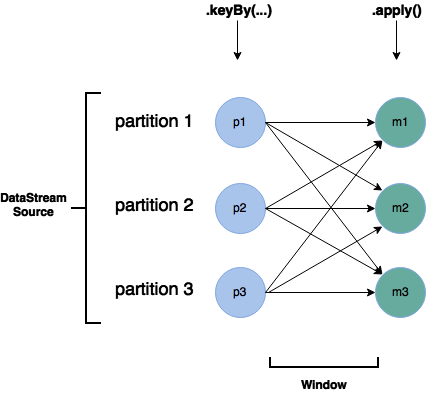
\includegraphics[scale=0.40]{img/ember_keyedstream}
	\caption{An example of Project Ember operation flow}
	\label{fig:ember_operation_flow}
\end{center}
\end{figure}


\section{DATA STREAM PROCESSING}

\subsection{Basic concepts}
Apache Flink is based on the concept of \texttt{DataStream} (it also supports datasets but they are not used in this project), which is an immutable collection of data where the number of elements is unbounded. 
DataStreams are produced by the \texttt{ExecutionEnvironment}, which is automatically created by the framework locally or distributed according to the cluster size defined in Flink configuration parameters. To create a data stream and to store it, the environment is bounded to a set of data \texttt{Sources} and \texttt{Sinks}.

In this project we needed to perform a real-time computation on several kinds of data sources, so we used the \texttt{DataStream API} made available by Apache Flink framework. This decision allowed us to create streams grouped by some specific attribute of the elements (as a \texttt{Key}), to aggregate them into \texttt{TimeWindows} and to perform later a \texttt{Join} operation to compute results on specific time intervals (\hyperref[fig:ember_keyedstream]{figure 2}).

Apache Flink is built to introduce very low latency for an high throughput and to allow the developers to create a natural flow control, decoupling the logic behind the stream processing from the deployment itself. In other words, it is built to be efficient and to let developers concentrate their efforts in building the topology of the system regardless the machines the system will run upon.

\subsection{Topology}
As we said, Apache Flink supports parallelism of the stream processing according to task slots available per-machine of its cluster. Describing the topology we will assume a certain degree of parallelism which is not necessary to run the system locally.

In \hyperref[fig:ember_topology]{figure 3} is represented the high level schema for our topology (except for the data sink, which updates the lamp's status in Elasticsearch). We can note that the streams produced are four: three coming from sensor sources attached to the execution environment (via Apache Kafka custom connectors) and one from a custom source that generates anomalies retrieved from queries to Elasticsearch lamps index and then perform a failure check, producing alerts messages.
It is interesting to note the replication of the most CPU-consuming tasks, as well as the \texttt{KeyBy} of streams tuples by a specific key to perform transformations and forwarding to dedicated operators.

As it is clear from the topology schema, we made use of time windows to buffer, aggregate and analyze specific time intervals of the streams. This introduced overhead, increasing the time spent by one record into the system, but it allowed us to reduce the jitter on output messages and to stabilize the entire control system: using windows we can easily compare datasets of the same dimensions and properties, decoupling the arrival from the service process of our operators network.

\begin{figure}
\begin{center}
	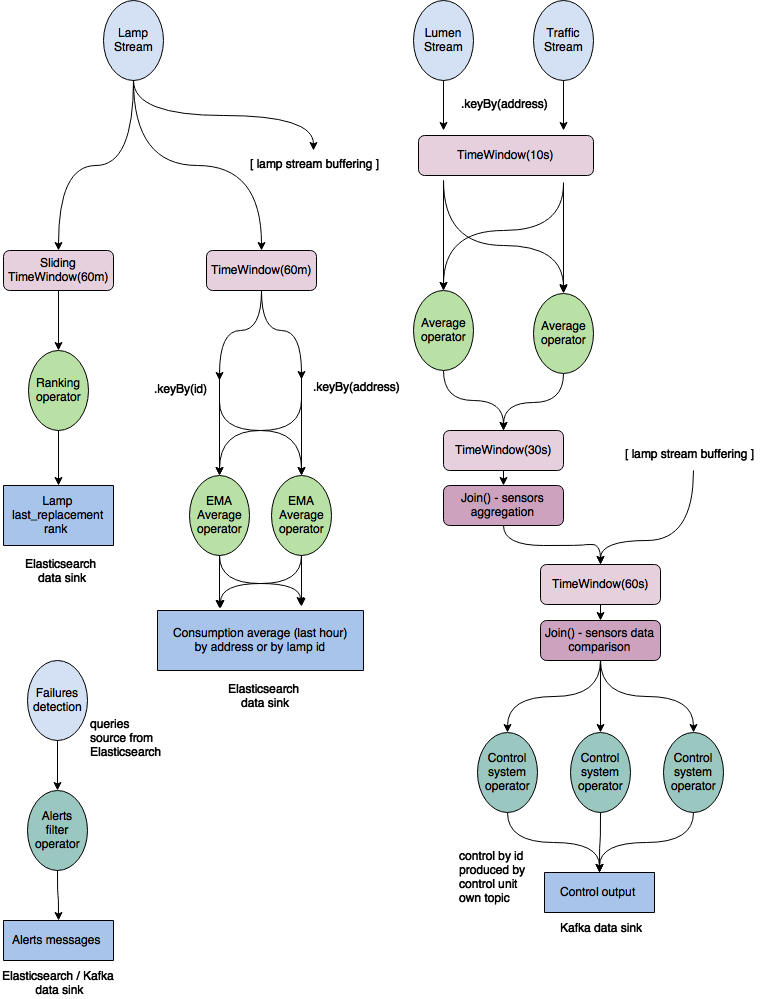
\includegraphics[scale=0.3]{img/ember_topology}
	\caption{Project Ember topology}
	\label{fig:ember_topology}
\end{center}
\end{figure}


\subsection{Sources and Sinks}
Sources are where the streams are injected into the processing system. \texttt{StreamExecutionEnvironment.addSource(sourceFunction)} can be used by the environment to attach sources to the topology - a similar API is provided for sinks. In particular a source function generates a \texttt{DataStream} that will be transformed and forwarded to the correct operators in the topology. We used as sources the Kafka connectors, available as Apache Flink plugins, to continuously consume from the topics \texttt{lamp, lumen, traffic} the records from the sensors, and a custom source function iterating over queries made to Elasticsearch in order to recover anomalies found in lamps history. Respectively we used the \texttt{FlinkKafkaConsumer010} to receive messages routed via the Kafka cluster and the customized \texttt{EmberElasticsearchAlertSource} which is powered by the tuple collector made available by the execution environment.

Sinks are, on the other hand, the way Apache Flink consumes the data streams and forward them to external systems or print them out in a file. In this implementation we used two custom sinks, extending the built-in connectors: one is the \texttt{EmberKafkaProducer} and the other is \texttt{EmberElasticsearchSinkFunction}. In particular the latter is extended for each use case, from the simple lamp history update operations to the update of the ranks of the life-expiring lamps. The first producer instead is a \texttt{SinkFunction} which is extended in the \texttt{EmberKafkaControlSink}: in this case we used the feature of the Java Kafka API to select and create a topic into the MOM, that was particularly useful to route, for each lamp, its control output, labeling each feedback with the lamp's own control unit identifier. An high level schema is represented in \hyperref[fig:ember_kafkatopology]{figure 4}.

\begin{figure}[!b]
\begin{center}
	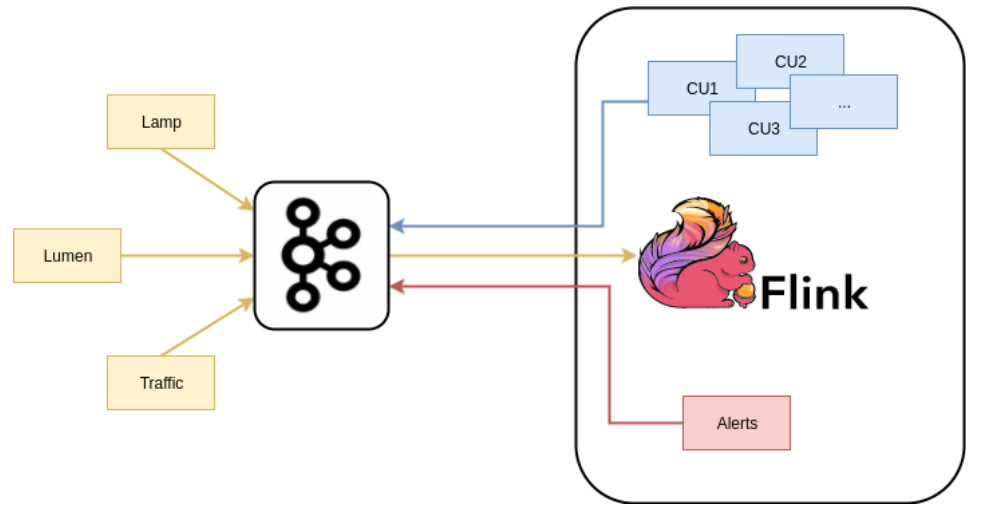
\includegraphics[scale=0.40]{img/ember_kafkatopology}
	\caption{Topics based messages routing}
	\label{fig:ember_kafkatopology}
\end{center}
\end{figure}


\subsection{Data aggregation}
The large part of our stream processing system is based upon \texttt{TumblingWindow} (\hyperref[fig:flink_windows]{figure 3}) and \texttt{KeyedStream}\footnote{Windows on keyed streams: https://ci.apache.org/projects/flink/flink-docs-release-1.2/dev/windows.html} classes. In fact, as we can see from our topology, the great part of the operators is composed of a keyed streams (grouped by an attribute of the records they collect) being windowed for an amount of time to compute over them a custom \texttt{JoinFunction}. There are exceptions, like the ranking and the alerting system and history-update by Elasticsearch sink, which don't require such a complexity and are simply buffered and iterated upon in order to collect new data streams. 

As we saw in the topology, we used a specific selector to partition the streams by ID, or address (\hyperref[fig:ember_operation_flow]{figure 4}). Then we will buffer the streams and their partitions according to a \texttt{Watermark} assigned by the source connector (typically the timestamp associated with the event generation), into windows which size is configurable. It is important to note here that the developer must pay attention to specify a \texttt{EventTimeTumblingWindow} for events generated from the source and not already processed by the system, and for records already processed a \texttt{ProcessingTimeTumblingWindow} in cascade. In particular, for a window following a previous aggregation (as it is for the control operator) we will use the \texttt{ProcessingTime} to maintain the system coherent with its internal clock and preserving the original event generation time assigned by watermarks definition.

Finally we can choose which operation is performed on collected records calling the \texttt{apply()} function, for example a moving average computation by lamp identifier or lamp address. We can also perform a \texttt{join()} over a new stream using a particular window in order to aggregate different data records in a single tuple and make them available for further operations, as it is performed twice in the control system flow.

\subsection{Project queries}
In this section we will cover each of the queries on which the system was designed and built\footnote{Italian project specs and original statement available at \url{http://www.ce.uniroma2.it/courses/sdcc1617/progetti/SDCC1617_progetto1.pdf}}.

\subsection*{Control system}
The core of the control system is the flow which takes the sensors data streams, buffers and aggregates them twice (by their common selector and with data from lamps) and produces a control output which is sent to Kafka cluster to be consumed by control units.

In particular, the light sensors and traffic records are partitioned via their address and then buffered into a 10 seconds (event time) window. This let the system behave according to a unique step: the ten-seconds-interval assumed in the project specifications. After that a simple arithmetic average is performed on the records received, before aggregating the two streams by their address attribute. Then a new 30 seconds (processing time) window is used to aggregate those new tuples with the raw data from the lamps and compare them. Every minute the control system filters the lamp by their IDs and produces optimal control values, using the formula:
	$$I = \frac{L_l*C_u}{A_l} \rightarrow L_l = I * A_l$$
	where the optimal intensity level (i.e. the lumen level per square meter), is proportional to an attenuation factor (assumed unitary in this implementation). Our control output is the lumen level.

	The optimal level is calculated via the previous formula, in addition to a comparison between the level measured from the lamp and the intensity from lumen sensors, and it is normalized using the percentage of traffic and safety limits. The idea is to achieve a trade-off between lamp consumption reduction (guaranteeing an optimal level of light in case of intense vehicles traffic) and a safety level for inhabited zones (securing pedestrian traffic as well). In addition, working on lumen sensors, we can achieve the goal to find an optimal value even in scarce weather conditions, according to light sensors readings (for example in a cloudy or rainy day).

Finally the output produced is a \texttt{DataStream<StreetLamp>} which is produced into a Kafka topic labeled by, for each lamp, its control unit alphanumeric identifier.

\subsection*{Statistics}
An important aspect of this project was to compute on the fly useful statistics on the smart city grid. We provided three different approaches for three different use cases.
\begin{itemize}
	\item \textbf{Expiration ranking} To produce an always updated rank of the ten (size is configurable) most in danger lamps (based on end-of-life expiration), we used an \texttt{EventTimeSlidingWindow} which takes care to perform a per-hour rank upon the last replacement (as a timestamp) attribute scanning the lamps records.
	\item \textbf{Last hour consumption} The system is also capable to track (based on a one-hour-interval) the average consumption, which is stored into Elasticsearch for security reasons (if the system is terminated or must be restarted the persistence level will take trace of the history, losing just the last hour measurements). To perform a computation which is focused on giving the most reasonable results, we used an exponential moving average:
$$S_t = \alpha*Y_t + (1 - \alpha)*S_{t-1}$$
where $\alpha$ is 0.8, giving preference to the last results from the hour-long buffer. The average is computed by address and by ID for further analysis: on Elasticsearch we can retrieve the per-day and per-week statistics, on single district or whole city, with no effort, simplifying the topology and making available the data to everyone accessing the persistence level.
	\item \textbf{Data history} An important aspect of a project like Project Ember is data visualization. Even if we already covered how Elasticsearch works and how Kibana is integrated, we want to remember that their use and a continuously updated history for the lamps values, as well as last hour consumptions, let us build useful dashboards to monitor in (near) real-time the system's overall status.
\end{itemize}

\begin{figure}[!b]
\begin{center}
	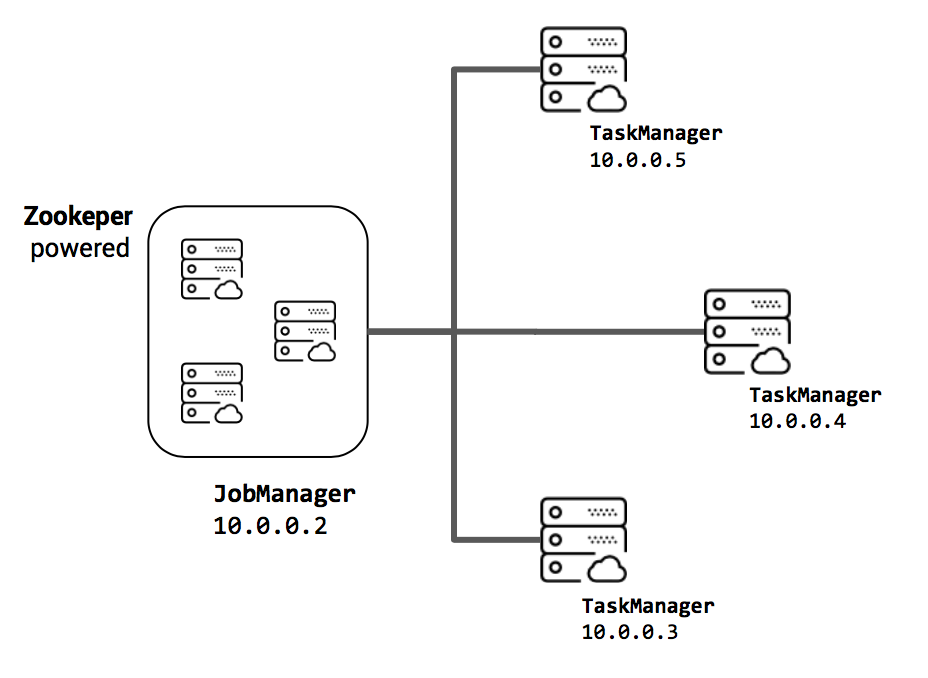
\includegraphics[scale=0.40]{img/ember_ha}
	\caption{Apache Flink distributed runtime (under HA)}
	\label{fig:ember_ha}
\end{center}
\end{figure}

\subsection*{Monitoring and Alerts generation}
A useful feature of Project Ember is to provide a customizable preferential access to the anomalies detection system. Once a configurable time (default is 30 seconds) is set, a query is performed to Elasticsearch cluster (using its Apache Lucene based core) to check on the entire lamps index for anomalies (e.g out of range luminosity levels, electrical failures or lamp life expiration overflowed limits): this produces a \texttt{DataStream<Alert>} via a custom \texttt{SinkFunction}. This stream is processed, analyzed and proper alerts messages are later produced in a new stream (according to the query results); they are later sent to a custom sink on Elasticsearch or Kafka clusters, according to the final user configuration (dashboard-based approach or not).

Finally the stream produced by Kafka source (reading the lamps' state) is also stored in Elasticsearch. This is particularly useful to visualize via Kibana the status of the entire system, providing real-time updates from all the grid. 

\subsection{Distributed runtime}
The cluster where Apache Flink runs can be configured to operate under HA\footnote{High Availability}, together with a distributed environment to ensure rebalancing of the operators amongst the cluster nodes: high level representation in \hyperref[fig:ember_ha]{figure 5}. 
In particular, it is necessary to set up how the \texttt{JobManager} and the \texttt{TaskManagers} cooperate. As we have seen, Apache Flink supports rebalancing on all the available computational slots of the system: the manager node is the one responsible to read the \texttt{.jar} and \texttt{.config} source files, producing the plan (thanks to the Flink framework) and redistributing into the slaves the computational effort. It can be achieved out of the box specifying in the framework configuration folder the IP addresses (or hostnames) of the slaves, where the \texttt{TaskManagers} reside, and the master's own, for each of the nodes. Running the cluster from the master will result in the creation of an overlay network\footnote{It could be necessary to specify \texttt{SSH} authentication credential when prompted}.

To ensure the HA the master node, where the \texttt{JobManager} resides, must be part of a Zookeeper quorum: this behaviour as well is supported out of the box by the framework.

\subsection{Configuration}
Most of the parameters we used to describe the stream's processing and control system are configurable via a \texttt{.properties} file. For a user guide please visit the project \href{https://github.com/projectember/project-ember}{repository}.

\begin{figure}
\begin{subfigure}{.5\textwidth}
	\centering
	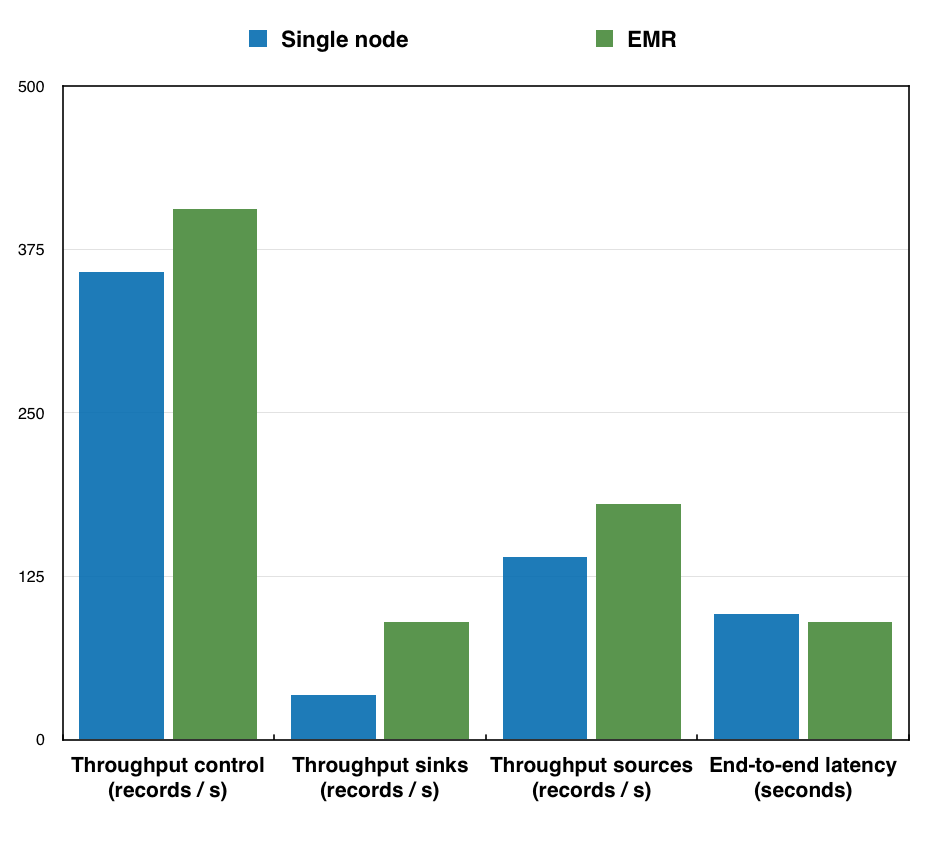
\includegraphics[scale=0.50]{img/ember_chart}
	\caption{Performances metrics comparison}
	\label{fig:ember_chart}
\end{subfigure}

\begin{subfigure}{.5\textwidth}
	\centering
	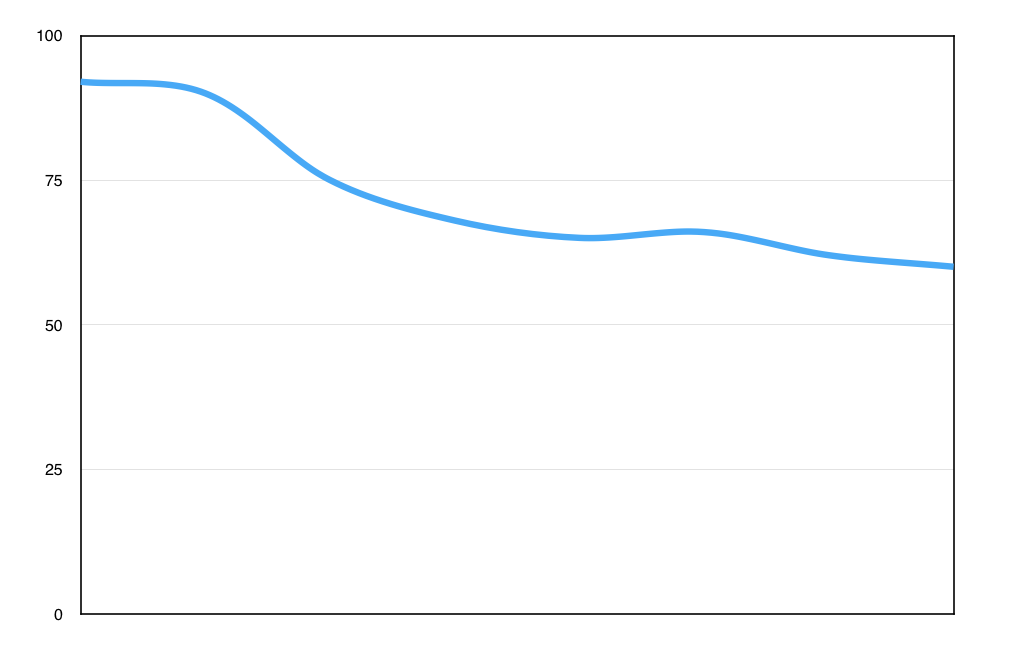
\includegraphics[scale=0.50]{img/ember_chart_latency}
	\caption{End-to-end latency (seconds) - transient analysis}
	\label{fig:ember_chart_latency}
\end{subfigure}
\caption{Project Ember operational performances}
\label{fig:ember_metrics}
\end{figure}


\section{TESTS AND PERFORMANCES}
It is clear that Project Ember has a lot of different metrics upon which performances analysis can be made . Proceeding with the validation of our architecture we conducted a lot of tests to ensure the forwarding operation between different operators in API concepts and in behavior (think of the difference between the Kafka consumer as a source, the alerts query on Elasticsearch, the Kafka producers as sinks etc.). In this section we will cover what we think are the most important metrics to face when deploying this system at scale, as well as the configuration we used to produce the data you can appreciate in \hyperref[fig:ember_metrics]{figure 6}.

\subsection{The city simulator}
There are two way to test a project of this kind: testing just the stream processing topology producing a fake data source or simulating the entire grid. The latter was our choice.

We developed a "city simulator", configurable and customizable: a multithreaded Python console application capable of simulating the behavior of thousands of lamps. The values produced are typical of a grid of lamps and sensors across a day-long span, with different lumen levels according to the height of the sun (via a simple sin wave), with random traffic percentage registered for each street, different values for bulbs' models and a rumored measure introduced to simulate consumption levels.

The simulator, codenamed Tomorrowland, sends to actually deployed control units data comparable with those of a small district of a typical Italian city. In particular, in the tests we will have two thousands lamps from one hundred different locations, transmitting to their control unit every ten seconds, and two thousands lumen level records sent directly to the Kafka cluster with one hundred records describing traffic average on the different streets. 

\subsection{Testing environment}
We adopted two configurations to test the architecture performances. Both of them used a replicated cluster of Apache Kafka nodes and a small cluster for Elasticsearch. Both of them were deployed using the AWS EC2 cloud service\footnote{Amazon Web Services, Elastic Compute Cloud - \url{aws.amazon.com/ec2}} offered by the Amazon Student Grant. Both the Apache Kafka cluster and the Elasticsearch one run with a three-node configuration using a general purpose tier, labeled by AWS as \texttt{m4.large}, with 2 vCPUs and 8 GB of memory, 450 Mbps in bandwidth. 

In particular, for the stream processing system we used two different approaches: a very powerful single node (and our local development machines during development) running Apache Flink and a cluster of nodes running in high-availability and managed via YARN on AWS Elastic Map Reduce\footnote{Elastic Map Reduce - \url{aws.amazon.com/emr}}. In the first the machine was labeled as \texttt{m4.xlarge}, 4 vCPUs and 16 GB of memory, for 750 Mbps in bandwidth. In the second case the EMR cluster was defined as formed by five machines - two for HA\footnote{High-Availability} for the JobManager and three for the TaskManagers -  every of them of the \texttt{m4.large} type.

To simulate the control unit, one of them was deployed on a Raspberry Pi 2 Model B to provide a sort of a dedicated-hardware for our testing environment.

\subsection{Metrics}
From the topology the most critical components were those that managed the control system. In particular the entire flow from the sensors sources to the final aggregation and data comparison operators. We made an extensive use of the Apache Flink web dashboard to retrieve data during the execution and compare them on an average basis (\hyperref[fig:ember_metrics]{figure 6}). From first monitoring sessions of the platform, the latency in forwarding the streams between the operators was below the \texttt{.001} seconds, so we concentrated our effort on the control system. 

The bottleneck was clearly the capacity of the Kafka consumers, that was why different levels of windows were made to filter and aggregate the records to optimize and "batch" the control system input. The latency of the end-to-end system, from the record generated by the control unit to the control output received via Apache Kafka, is stable due to network performances which are the same for each configuration. We noted that the throughput in the control system is not largely influenced by the increased parallelism of the TaskManagers, even if we have a slight enhancement. We observed however a large improvement in the throughput of the Kafka producers in the end of the control system, which proved an increased responsiveness and a reduced latency. 

It is interesting to analyze the transient period from the starting-up of the control system to the stability. The one-minute-and-thirty-seconds-large window to aggregate data and produce an optimal control feedback, on the very first run is actually the end-to-end latency measured. When the system is stable, the latency decreases until reaching a one-minute response time. This is due to the particular configuration of the windows we described, which made the system capable of figuring out an optimal control every minute basing its decision on a small part of the historical data from the lamps - the multiple windows levels aggregation.

It is clear that the statistics output will be delayed by the windows size (which is one-hour-long), with a five-millis-long maximum computation time. However this latency is not significant for the system reactivity.

\section{NEXT STEPS AND CONCLUSIONS}

\subsection{Security}
The control unit has the role of lamp validator, so it can grant access to those lamps that have been registered by an operator on the unit itself. Kafka on the other way can be customized using different security protocol (SSL primarily); control units can be trusted and verified and they guarantee for the lamps registered by them. An API key can be provided to trusted devices that can register new lamps to control unit thanks to AWS Lambda. 

\subsection{Deployment}
All the components we described have also been tested on Docker. Create a simple container is easy but relate one to another in order to create a cluster was not easy as well. Docker remains a valuable asset for deploying all of these components with a single instruction to lunch and manage the cluster. Components such as Elasticsearch and Kafka can be scaled at runtime by adding or removing nodes; the system is prone to be autonomic with a contained amount of effort.

Moreover, fine pre-production tuning on the cluster can be made to decrease the windows size in order to increase the system reactivity to small changes in the illumination system.

\subsection{Conclusions}
Project Ember was developed keeping in mind the necessities of a modern city. So we tried to provide where possible a plug-and-play solution, for example with the city grid architecture, and scalability-enabled architectural choices where it was necessary to deploy a larger cluster. We believe Project Ember is ready to be tested on a larger environment, using a real scenario typical values to tune the different components and their cooperation. 

\section*{Repository}
The Project Ember official homepage, with guides and code to deploy and customize each component described in this paper, is available at: \href{https://github.com/projectember}{github.com/projectember}. Fork us!
